% !TEX root = ../main_lecture_notes.tex
\chapter{Marche aléatoire et Martingale à temps discret}\label{chap:marche_aléatoire}
Ce cours propose une introduction au calcul stochastique avec pour application principale la modèlisation des marchés financiers et la gestion des risque en assurance. L'objet d'étude principale sont les processus stochastique. 
\begin{definition}\label{def:filtration}
Soit $(\Omega, \F, \Prob)$ un espace probabilisé. Une suite $(X_t)_{t\geq0}$ de variable aléatoires (\va) sur $\Omega$ est un processus stochastiques.
  \begin{itemize}
    \item Si $t\in \N$ alors $(X_t)_{t\geq0}$ est un processus stochastique à temps discret. Par exemple une chaine de Markov. 
    \item si $t\in \RL_+$ alors $(X_t)_{t\geq0}$ est un processus stochastique à temps continu. Par exemple le processus de Poisson. 
  \end{itemize}
\end{definition}
% L'utilisation des processus stochastiques pour comprendre le comportements des actifs financiers date des travaux de Bachelier. Près de 70 ans plus tard, Samuelson (prix nobel d'économie en 1970) proposa l'utilisation du mouvement Brownien avec drift. La théorie moderne repose sur les modèles de Black, Scholes and Merton, ce qu'on appelle la théorie des options et les arguments d'absence d'opportunité d'arbitrage. 
\section{La marche aléatoire et le problème de la double dépense}
\subsection{Blockchain, cryptomonnaie et double dépense}
Une blockchain est une base de données constituée de blocs successifs maintenue par un réseau pair-à-pair, comme sur la \cref{fig:blockchain_network}. 
\begin{figure}[ht!]
\begin{center}
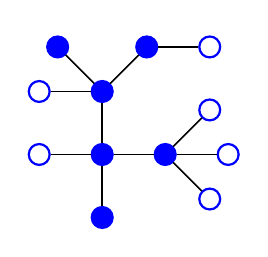
\begin{tikzpicture}[-, >=, auto, semithick, node distance=01cm]
\tikzstyle{every edge}=[segment length=1mm,segment angle=10, draw]

\tikzstyle{full node}=[circle, fill=blue,draw=blue,thick,text=black,scale=0.8]
\tikzstyle{light node}=[circle, fill=white,draw=blue,thick,text=black,scale=0.8]
\node[full node]    (1)                     {};
\node[full node]    (2)[above right of=1]         {};
\node[full node]    (3)[above left of=1]         {};
\node[full node]    (4)[below of=1]         {};
\node[full node]    (5)[right of=4]         {};
\node[full node]    (6)[below of=4]         {};
\node[light node]    (7)[left of=1]         {};
\node[light node]    (8)[right of=2]         {};
\node[light node]    (9)[left of=4]         {};
\node[light node]    (10)[above right of=5]         {};
\node[light node]    (11)[ right of=5]         {};
\node[light node]    (12)[ below right of=5]         {};
% \node[light node]    (4)[above of=2]         {};
\path

(1) edge node{} (2)
    edge node{} (3)
    edge node{} (7)
    ;
\path
(5) edge node{} (10)
    edge node{} (11)
    edge node{} (12)
    ;
    \path
(4) edge node{} (5)
    edge node{} (1)
    edge node{} (9)
    edge node{} (6)
    ;
    \path
(2) edge node{} (8)   
    ;
\end{tikzpicture}
\end{center}
\caption{Un réseau fait de noeuds lourds (bleu) et de noeuds légers (blanc)}
\label{fig:blockchain_network}
\end{figure}
Les noeuds légers se contentent d'émettre des informations (appelées transactions). Les noeuds lourds doivent vérifier la cohérence des transactions et s'accorder sur les informations à inscrire dans la blockchain. Les noeuds lourds appliquent un protocole de consensus pour se mettre d'accord. La preuve de travail ou \textit{Proof-of-Work} est le protocole utilisé dans le cadre de la blockchain des bitcoins, voir le whitepaper de \citet{Nakamoto2008}. Un bloc doit être ajouté toutes les dix minutes environ, les noeuds sont en compétition pour résoudre un problème cryptographique brutalement via une méthode essai-erreur (\textit{trial and error}). Le premier qui parvient à résoudre le problème ajoute le bloc et récupère une récompense d'un montant de BTC$6.25$ à l'heure de l'écriture.\footnote{\url{https://bitcoinblockhalf.com/}}. \\

Dans la blockchain des bitcoins, les informations enregistrées sont des échanges de bitcoin entre les participants. Un noeud peut facilement émettre deux transactions conflictuelles, c'est à dire qui transfèrent les mêmes unités à deux entités différentes. Il s'agit d'une attaque par double dépense. Le scénario standard est le suivant:
\begin{enumerate}
    \item Marie transfère à John BTC$10$
    \item La transaction de Marie à John est enregistrée dans la blockchain
    \item John doit atendre $\alpha\in\N$ confirmations, c'est à dire que $\alpha-1$ blocs soient ajouté après celui dans lequel la transaction de Marie à John est inscrite
    \item Une fois que $\alpha$ confirmations ont été envoyées, John envoie le bien à Marie
    \item Pendant ce temps, Marie travaille sur sa propre version de la blockchain (dite privée) dans laquelle la transaction de Marie à John est remplacée par une transaction de Marie à elle même
    \item Au moment de la livraison du bien la blockchain dite principale est en avance de $z$ blocs 
    \item L'objectif de Marie est générer une chaine concurrente plus longue que la chaine principale. Si elle y parvient, elle la communiquera à l'ensemble du réseau pour créer une fourche (\textit{fork}). Le réseau optera alors pour la branche la plus longue.
    La branche de Marie va alors remplacer la branche principale permettant à Marie de récupérer ses unités qu'elle peut dépenser à nouveau. 
\end{enumerate}
Cette course entre les deux branches est résumée sur la \cref{fig:dp_illustration}.
\begin{figure}[ht!]
\begin{center}
\begin{tikzpicture}[-, >=stealth', auto, semithick, node distance=1cm]
% \tikzstyle{block} = [rectangle, draw, fill=blue!20,
%     text width=5em, text centered, rounded corners]
\tikzstyle{block}=[rectangle, fill=black,draw=black,thick,text=black,scale=1.5]
\tikzstyle{block}=[rectangle, fill=white,draw=black,thick,text=black,scale=1.5]
\tikzstyle{confirmed block}=[rectangle, fill=white,draw=blue,thick,text=black,scale=1.5]
\tikzstyle{bad block}=[rectangle, fill=white,draw=red,thick,text=black,scale=1.5]
\node[block]    (1)                     {\tiny $\text{M}\rightarrow \text{J}$};
\node[block]    (2)[right of=1]                     {};
\node[block]    (3)[right of=2]                     {};
\node[block]    (4)[right of=3]                     {};
\node[confirmed block]    (5)[right of=4]                     {};

\node[bad block]    (6)[below of=1]         {\tiny $\text{M}\rightarrow \text{M}$};
\node[block]    (7)[right of=6]         {};
\node[block]    (8)[right of=7]         {};
\path
(1) edge[ left]     node{}     (2)
(2) edge[ left]     node{}     (3)
(3) edge[ left]     node{}     (4)
(4) edge[ left]     node{}     (5)
(6) edge[ left]     node{}     (7)
(7) edge[ left]     node{}     (8);

\end{tikzpicture}
\end{center}
\caption{La course à la double dépense illustrée, ici nous avons $\alpha = 4$ et $z = 2$}
\label{fig:dp_illustration}
\end{figure}
Notre objectif est de caluler la probabilité que la branche de Marie devienne majoritaire. Pour ce faire nous allons construire un modèle mathématique.
\subsection{La marche aléatoire sur $\Z$}
Soit $(Z_n)_{n\in\mathbb{N}}$ la différence de longueur entre la branche de Marie et la branche principale de la blockchain. On a $Z_0 = z\geq 0$ et la double dépense se produit à l'instant aléatoire
\begin{equation}\label{eq:dp_time}
\tau_0 = \inf\{n\geq0\text{ ; }Z_n = 0\}.
\end{equation}
Nous souhaitons étudié la distribution de $\tau_0$ et en particulier calculer la probabilité de double dépense définie par 
\begin{equation}\label{eq:dp_prob}
\phi(z) = \Prob(\tau_0 <\infty|Z_0 = z) := \Prob_z(\tau_0 <\infty)
\end{equation}
A chaque instant $k\in\N$ un bloc est ajouté, il appartient 
\begin{itemize}
    \item A la branche principale avec probabilité $p\in(0,1)$
    \item à la branche de Marie avec probabilité $1-p$
\end{itemize}
Soit $(\Omega,\F, \Prob)$ un espace probabilisé. On définit une suite $(\xi_n)_{n\geq0}$ \iid de variables aléatoires (\va) de loi 
$$
\mathbb{P}(\xi = 1) = p\text{, et }\mathbb{P}(\xi = 1) = 1-p.
$$
On en déduit que 
$$
Z_n = z +\sum_{k=1}^n\xi_k.
$$
Le processus $Z_n$ est un processus à temps discret et à valeur dans $\Z$. Une visualisation du problème de premier passage est donné sur la \cref{fig:double_spending_time}.
\begin{figure}[ht!]
\begin{center}
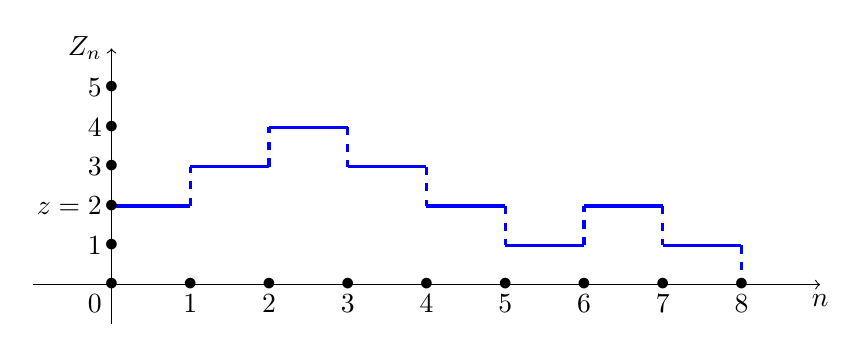
\begin{tikzpicture}
  %Origin and axis
  \coordinate (O) at (0,0);
  \draw[->] (-1,0) -- (9,0) coordinate[label = {below:$n$}] (xmax);
  \draw[->] (0,-0.5) -- (0,3) coordinate[label = {left:$Z_n$}] (ymax);
  %Lower linear boundary

 
  %Stochastic process trajectory
  
  \draw (0,0) node[blue,left] {} node{};
  \draw[very thick,blue,-] (0,1) -- (1,1) node[pos=0.5, above] {} ;
  \draw[very thick,dashed,blue] (1,1) -- (1,1.5) node[pos=0.5, right] {};
  \draw[very thick,blue,-] (1,1.5) -- (2,1.5) node[pos=0.5, above] {};
  \draw[very thick,dashed,blue] (2,1.5) -- (2,2) node[pos=0.5, right] {};
  \draw[very thick,blue,-] (2,2) -- (3,2) node[pos=0.5, above] {};
  \draw[very thick,dashed,blue] (3,2) -- (3,1.5) node[pos=0.5, right] {};
  \draw[very thick,blue,-] (3,1.5) -- (4,1.5)node[pos=0.5, above] {};
  \draw[very thick,dashed,blue] (4,1.5) -- (4,1) node[pos=0.5, right] {};  
  \draw[very thick,blue,-] (4,1) -- (5,1) node[pos=0.5, above] {};
  \draw[very thick,dashed,blue] (5,1) -- (5,0.5) node[pos=0.5, right] {};  
  \draw[very thick,blue,-] (5,0.5) -- (6,0.5) node[pos=0.5, above] {};
  \draw[very thick,dashed,blue,-] (6,0.5) -- (6,1) node[pos=0.5, above] {};
   \draw[very thick,blue,-] (6,1) -- (7,1) node[pos=0.5, above] {};
    \draw[very thick,dashed,blue,-] (7,1) -- (7,0.5) node[pos=0.5, above] {};
     \draw[very thick,blue,-] (7,0.5) -- (8,0.5) node[pos=0.5, above] {};
     \draw[very thick,dashed,blue,-] (8,0.5) -- (8,0) node[pos=0.5, above] {};
  %Jump Times
  \draw (1,0) node[black,below] {$1$} node{ \color{black}$\bullet$};
  \draw (2,0) node[black,below] {$2$} node{ \color{black}$\bullet$};
  \draw (3,0) node[black,below] {$3$} node{ \color{black}$\bullet$};
  \draw (4,0) node[black,below] {$4$} node{ \color{black}$\bullet$};
  \draw (5,0) node[black,below] {$5$} node{ \color{black}$\bullet$};
  \draw (6,0) node[black,below] {$6$} node{ \color{black}$\bullet$};
  \draw (7,0) node[black,below] {$7$} node{ \color{black}$\bullet$};
  \draw (8,0) node[black,below] {$8$} node{ \color{black}$\bullet$};
  %Level of the counting process
   \draw (0,0) node[black,below left] {$0$} node{ \color{black}$\bullet$};
   \draw (0,0.5) node[black,left] {$1$} node{ \color{black}$\bullet$};
   \draw (0,1) node[black,left] {$z=2$} node{ \color{black}$\bullet$};
   \draw (0,1.5) node[black,left] {$3$} node{ \color{black}$\bullet$};
   \draw (0,2) node[black,left] {$4$} node{ \color{black}$\bullet$};
   \draw (0,2.5) node[black,left] {$5$} node{ \color{black}$\bullet$};

  % %Aggregated Capital gains
%  \draw (0,1.5) node[blue,below right] {$\mu_1$} node{ \color{blue}$-$};
%  \draw (0,2.25) node[blue,left] {$\mu_2$} node{ \color{blue}$-$};
%  \draw (0,3.75) node[blue,left] {$\mu_3$} node{ \color{blue}$-$};
  %Ruin time = First-crossing time time
%  \draw (5,0) node[black,above right] {${\tau_0}_u$} node{ \color{black}$\times$};
%  \draw[dotted,black] (0,3.28) -- (5,3.28);
%  \draw[dotted,black] (5,0) -- (5,3.28);
\end{tikzpicture}
\end{center}
\caption{Illustration du problème de premier passage sous-jacent à la double dépense.}
\label{fig:double_spending_time}
\end{figure}

Le processus $Z$ est la marche aléatoire sur $\Z$. Ce processus est une chaine de Markov.
\subsection{Filtration, chaine de Markov et temps d'arrêt}
Soit $(\Omega,\F, \Prob)$ un espace probabilisé sur lequel on définit un processus $X:=(X_n)_{n\geq0}$. 
\begin{definition}\label{def:filtration}
Une filtration $(\F_n)_{n\geq0}$ est une suite de sous-tribu de $\F$, croissante pour l'inclusion au sens où
$$
\F_k\subset \F_n,\text{ pour }k\leq n.
$$

\end{definition}
$\F_n$ correspond à l'information disponible au temps $n$. C'est aussi l'information nécessiare pour tracer la trajectoire du processus jusqu'à l'instant $n$.
\begin{definition}\label{def:processus_adapte}
Le processus X est $\F_n$-adapté si $X_n$ est mesurable par rapport $\F_n$. La suite
$$
\F_n = \sigma(X_1,\ldots, X_n),\text{ }n\in \N,
$$ 
est la filtration naturelle du processus $X$.
\end{definition}
\begin{ex}\label{ex:filtration_marche_aleatoire}
La marche aléatoire $Z_n$ est adaptée à la filtration $$
\F_n = \sigma(\xi_k,\text{ }k\leq n).
$$
\end{ex}
Soit un processus $X:=(X_n)_{n\geq0}$ adapté à la filtration $(\F_n)_{n\geq0}$ à valeur dans l'espace d'état $E$.
\begin{definition}\label{def:CM}
Le processus $X$ est une chaine de Markov sur un espace d'état $E$ si pour toute fonction mesurable $g:E\mapsto \RL$,
$$
\E[g(X_n)|\F_{n-1})] = \E[g(X_n)|X_{n-1}].
$$
Si de plus 
$$
\E[g(X_n)|X_{n-1})] = \E[g(X_1)|X_0]
$$
alors $X$ est une chaine de Markov homogène (CMH).
\end{definition}
Une CMH est caractérisée par son espace d'état, sa loi initiale 
$$
\mu(x) = \Prob(X_0 = x),
$$
et ses probabilités de transitions notées
$$
p(x,y) = \Prob(X_{n+1} = y|X_{n}= x),\text{ pour tout }n\geq0\text{ et }(x,y)\in E^2.
$$
On notera $\Prob_x(\cdot)$ et $\E_x(\cdot)$ la probabilité et l'espérance conditionnelle sachant $X_0 = x$. 

\begin{prop}
Soit $(\xi_n)_{n\geq1}$ une suite de \va \iid et indépendante de la \va $X_0$ à valeur dans $E$. Le processus
$$
X_n = F(X_{n-1}, \xi_n),\text{ }n\geq1,
$$
pour toute fonction mesurable $F:E\times G\mapsto E$ est une CMH.
\end{prop}
\begin{ex}
On observe que la marche aléatoire $Z$ vérifie
$$
Z_{n} = Z_{n-1} + \xi_{n},\text{ }n\geq1.
$$
Il s'agit bien d'une CMH dont les probabilités de transitions sont données par 
$$
p(x,y) = \begin{cases}
p&\text{ si }y = x+1,\\
1-p&\text{ si }y = x-1,\\
0& \text{ sinon}.
\end{cases}
$$
\end{ex}
\begin{definition}\label{def:temps_arret}
Une variable aléatoire $\tau:\Omega\mapsto \overline{\RL}_+ = \RL_+\cup{+\infty}$ est un temps d'arrêt pour le processus $X$ et sa filtration $(\F_n)_{n\geq0}$ si 
$$
\{\tau\leq n\}\in \F_n\text{, pour tout }n\geq1.
$$
\end{definition}
\begin{ex}\label{ex:dp_time}
Le temps de double dépense $\tau_0 = \inf\{n \geq0\text{ ; }Z_n = 0\}$ est un temps d'arrêt du processus $Z$. En effet, on peut écrire 
$$
\{\tau_0=n \} = \bigcap_{k=1}^{n-1}\{Z_k\neq 0\}\cap\{Z_n = 0\}.
$$
\end{ex}

\begin{definition}\label{def:markov_forte}
Un processus $X$ vérifie la propriété de Markov forte si pour $\tau$ un temps d'arrêt et $g:E\mapsto \RL$ mesurable, on a 
$$
\E[g(X_{\tau + n})|\F_\tau]= \E[g(X_{\tau + n})|X_\tau].
$$
\end{definition}
Une CMH $X$ vérifie la propriété de Markov forte. En fait, pour temps d'arrêt fini presque surement, la chaine de Markov $\tilde{X}=(X_{n+\tau})_{n\geq0}$ a les mêmes caractéristiques que $X$. C'est à dire même espace d'état et probabilités de transition, seule la loi initiale diffère avec
$$
\tilde{\mu}(x) = \Prob(\tilde{X}_0 = x) = \Prob(X_\tau = x).
$$ 
L'étude des temps d'arrêt comme $\tau_0$ procède de l'analyse à un pas décrite dans le résultat suivant. 
\begin{prop}
Soit $\tau_A=\inf\{n\geq0\text{ ; }X_n\in A\}$, avec $A\subset E$ tel que $\E_x(\tau_A)<\infty$ pour tout $x\in E$. Soit $x\in E$ et $n\geq1$, alors
\begin{enumerate}
\item
$$
\Prob_x(\tau_A=n)=
\begin{cases}
0,&\text{ }x\in A,\\
\sum_{y\in E}p(x,y)\Prob_y(\tau_A=n-1),&x\notin A.
\end{cases}
$$
\item
$$
\E_x(\tau_A)=
\begin{cases}
0,&\text{ }x\in A,\\
1+\sum_{y\in E}p(x,y)\E_y(\tau_A),&x\notin A.
\end{cases}
$$
\end{enumerate}
\end{prop}
\begin{proof}
\begin{enumerate}
    \item Si $x\in A$ alors $\tau_A = 0$ $\Prob_x$-p.s. donc
    $\Prob_x(\tau_A=n)=0\text{ pour }n\geq1\text{ et }\Prob_x(\tau_A=0)=1$.
    Supposons $n = 1$ alors
    \begin{eqnarray*}
        \Prob_x(\tau_A=1)&=&\Prob(\tau_A=1|X_0=x)\\
        &=&\sum_{y\in E} \Prob(\tau_A=1, X_1=y|X_0=x)\\
        &=&\sum_{y\in A} \Prob(\tau_A=1 |X_1=y,X_0=x)p(x,y) \\
        &+& \sum_{y\in E/A} \Prob(\tau_A=1|X_1=y,X_0=x)p(x,y)\\
        &=&\sum_{y\in A} 1\times  p(x,y) + 0.\\
    \end{eqnarray*}
    On remplace $1$ par $\Prob_y(\tau_A=0)$ (=1 si $y\in A$), il vient
    $$
    \Prob_x(\tau_A=1)= \sum_{y\in A} \Prob_y(\tau_A=0)\times  p(x,y)
    $$
    quite à ajouter $0$ on a
    \begin{eqnarray*}
    \Prob_x(\tau_A=1)&=& \sum_{y\in A} \Prob_y(\tau_A=0)\times  p(x,y) + 0\\
     &=&\sum_{y\in A} \Prob_y(\tau_A=0)\times  p(x,y)\\
     &+& \sum_{y\in E/A} \Prob_y(\tau_A=0)\times  p(x,y).
    \end{eqnarray*}
    puisque $\Prob_y(\tau_A=0) = 0$ si $y\in E/A$. On vérifie bien que
    $$
    \Prob_x(\tau_A=n)=\sum_{y\in E}p(x,y)\Prob_y(\tau_A=n-1)\text{ pour }n = 1.
    $$
    Supposons $n>1$ alors
    \begin{eqnarray*}
    \Prob_x(\tau_A=n)&=&\Prob(\tau_A=n|X_0=x)\\
    &=&\sum_{y\in E} \Prob(\tau_A=n, X_1=y|X_0=x)\\
    &=&\sum_{y\in A} \Prob(\tau_A=n |X_1=y,X_0=x)p(x,y) \\
    &+& \sum_{y\in E/A} \Prob(\tau_A=n|X_1=y,X_0=x)p(x,y)\\
    &=& 0+ \sum_{y\in E/A} \Prob(\tau_A=n|X_1=y,X_0=x)p(x,y)\\
    &=&  \sum_{y\in E/A} \Prob\left(\bigcap_{i = 0}^{n-1}\{X_i\notin A\}\cap\{X_n\in A\}|X_1=y,X_0=x\right)p(x,y)\\
    \end{eqnarray*}
    Sachant $\{X_0 = x\}$ l'évènement $\{X_0 \notin A\}$ est presque sûr. On a donc
     $$
     \Prob_x(\tau_A=n)=  \sum_{y\in E/A} \Prob\left(\bigcap_{i = 1}^{n-1}\{X_i\notin A\}\cap\{X_n\in A\}|X_1=y\right)p(x,y)
     $$
     On perd le conditionnement par rapport à $X_0$ car sachant $X_1$
     $$
     \bigcap_{i = 1}^{n-1}\{X_i\notin A\}\cap\{X_n\in A\}\text{ est indépendant de } X_0.
     $$
     Puis on remarque que comme $(X_n)_n\in \N$ est une CMH alors
     $$
     [(X_1, X_2,\ldots, X_n)|X_1  =y]\overset{\mathcal{D}}{=}[(X_0, X_1,\ldots, X_{n-1})|X_0 = y].
     $$
     Cela permet d'écrire
    \begin{eqnarray*}
    \Prob_x(\tau_A=n)&=&\sum_{y\in E/A} \Prob_y\left(\bigcap_{i = 0}^{n-2}\{X_i\notin A\}\cap\{X_{n-1}\in A\}\right)p(x,y)\\
    &=&\sum_{y\in E/A} \Prob_y\left(\tau_A = n-1\right)p(x,y) + 0\\
    &=&\sum_{y\in E} \Prob_y\left(\tau_A = n-1\right)p(x,y).
    \end{eqnarray*}
    \item Si $x\in A$ alors $\E_x(\tau_A)=0$ et sinon
\begin{eqnarray*}
\E_x(\tau_A)&=&\sum_{n=0}^{+\infty}n\times\Prob_x(\tau_A=n)\\
&=&\sum_{n=1}^{+\infty}n\sum_{y\in E}\Prob_y(\tau_A=n-1)p(x,y)\\
&=&\sum_{y\in E}p(x,y)\sum_{n=0}^{\infty}(n+1)\Prob_y(\tau_A=n)\\
&=&\sum_{y\in E}p(x,y)(1+ \E_y(\tau_A))\\
&=&1+\sum_{y\in E}p(x,y)\E_y(\tau_A).
\end{eqnarray*}

\end{enumerate}
\end{proof}
\begin{theo}
Si $p>1/2$ alors 
$$
\phi(z) = \left(\frac{1-p}{p}\right)^z.
$$
\end{theo}


\begin{proof}
Via un analyse à un pas, nous avons 
\begin{equation}\label{eq:difference_equation}
\phi(z) = p\phi(z+1)+(1-p)\phi(z-1),\text{ }z\geq1.
\end{equation}
Les conditions aux bords indiquent que 
\begin{equation}\label{eq:boundary_conditions_double_spending}
\phi(0) = 1\text{ and }\underset{z\rightarrow +\infty}{\lim}\phi(z) = 0
\end{equation}
L'équation \eqref{eq:difference_equation} défini une suite linéaire récurrente d'ordre $2$. L'équation caractéristique s'écrit
$$
px^2 - x + 1-p = 0.
$$
elle admet deux racines réelles
$$
r_1 = 1, \text{ and }r_2 = \frac{1-p}{p}.
$$
Les solutions de \eqref{eq:difference_equation} sont données par 
$$
\phi(z)=A+B\left(\frac{1-p}{p}\right)^z,
$$
où $A$ et $B$ sont des constantes. Grâce aux conditions initiales \eqref{eq:boundary_conditions_double_spending}, nous déduisons que
$$
\phi(z) = \left(\frac{1-p}{p}\right)^z,
$$
comme annoncé.
\end{proof}
Il est aussi possible de donner la loi de probabilité de $\tau_0$ via le résultat suivant.
\begin{theo}
Si $z = 0$ alors $\tau_0=0$ \ps. Si $z>0$ alors la loi de $\tau_0$ est donnée par
$$
\mathbb{P}_z(\tau_0 = n)=
\frac{z}{n}\binom{n}{(n-z) / 2}p^{(n-z) / 2}(1-p)^{(n
+z) / 2}\text{ si }n\geq z\text{ et }n-z\text{ est pair},
$$
et $0$ sinon.
\end{theo}
\begin{proof}
Nous avons besoin du lemme suivant.
\begin{lemma}\label{lem:markov_hitting_time}
\begin{equation}\label{eq:markov_hitting_time}
\mathbb{P}_z(\tau_0 = n) = \frac{z}{n}\mathbb{P}_z(Z_n = 0).
\end{equation}
\end{lemma}
\begin{proof}
Si $z = 0$ alors $\tau_0 = 0$ \ps et les deux membres \eqref{eq:markov_hitting_time} sont égaux à $0$. Supposons que $z\geq1$, nous avons $\mathbb{P}_z(\tau_0 = n) = 0$ et $\mathbb{P}_z(Z_n = 0) = 0$ lorsque $n<z$ et $n-z$ est impair. On raisonne par récurrence sur $n\geq1$, quand $n = 1$ nous avons
$$
\mathbb{P}_z(\tau_0 = 1) = 0 = \frac{z}{1}\mathbb{P}_z(Z_1 = 0),\text{ for }z>1, 
$$
et 
$$\mathbb{P}_1(\tau_0 = 1) = q = \frac{1}{1}\mathbb{P}_1(Z_1 = 0),\text{ for }z=1. 
$$
La propiété est vérifiée pour $n=1$. Supposons qu'elle soit vérifiée au rang $n>1$. En vertu de la loi des probabilités totales, nous avons 
\begin{eqnarray*}
\mathbb{P}_z(\tau_0 = n+1)&=&\sum_{y\in\{-1,1\}}\mathbb{P}_z(\tau_0 = n+1|\xi_1 = y)\mathbb{P}(\xi_1 = y)\\
&=&\sum_{y\in\{-1,1\}}\mathbb{P}_{z+y}(\tau_0 = n)\mathbb{P}(\xi_1 = y)\\
&=&\sum_{y\in\{-1,1\}}\frac{z+y}{n}\mathbb{P}_{z+y}(Z_n = 0)\mathbb{P}(\xi_1 = y)
\end{eqnarray*}
Pour la deuxième égalité, nous avons eu recours à la propriété de Markov forte. Nous "détricottons" la loi des probabilités totales pour obtenir
\begin{eqnarray}
\mathbb{P}_z(\tau_0 = n+1)&=&\sum_{y\in\{-1,1\}}\frac{z+y}{n}\mathbb{P}_{z}(\xi_1 = y|Z_{n+1} = 0)\mathbb{P}_z(Z_{n+1} = 0)\nonumber\\
&=&\frac{\mathbb{P}_z(Z_{n+1} = 0)}{n}\left[z+\mathbb{E}_z(\xi_1|Z_{n+1}=0)\right]\label{eq:law_total_probability_undone}
\end{eqnarray}
Comme les $Y_i$ sont \iid alors il vient 
$$
\mathbb{E}_z(\xi_1|Z_{n+1}=0) = \mathbb{E}_z(\xi_i|Z_{n+1}=0)\text{, } i = 1, \ldots, n+1,
$$
et par suite 
$$
\mathbb{E}_z(\xi_1|Z_{n+1}=0) = \frac{1}{n+1}\sum_{i =1}^{n+1}\mathbb{E}_z(\xi_i|Z_{n+1}=0) = \frac{-z}{n+1}.
$$
En injectant l'expression ci-dessus dans \eqref{eq:law_total_probability_undone}, il vient 
$$
\mathbb{P}_z(\tau_0 = n+1) = \frac{z}{n+1}\mathbb{P}_z(Z_{n+1} = 0).
$$
\end{proof}
Pour compléter la preuve, on remarque simplement que
$$
\mathbb{P}_z(Z_n = 0) = \binom{n}{(n-z) / 2}p^{(n-z) / 2}q^{(n
+z) / 2}.
$$
Il s'agit de la probabilité d'occurence d'une trajectoire de $(Z_n)_{n \geq0}$ commençant au niveau $Z_0 = z$ finissant au niveau $0$ comprenant $(n-z)/2$ sauts vers le haut et $(n+z)/2$ sauts vers le bas.
\end{proof}
\subsection{Loi invariante, récurrence et loi stationnaire}
Soit $(X_{n})_{n\in\N}$ une chaine de Markov homogène d'espace d'état $E$. 
\begin{definition}[Loi invariante]
Soit $\mu$ une loi de probabilité sur $E$. $\mu$ est une loi invariante si 
$$
\mu(y) = \sum_{x\in E}\mu(x)p(x,y),
$$
soit matriciellement $$\mu = \mu \mathbf{P}.$$
\end{definition}
\begin{definition}[Loi réversible]
Soit $\lambda$ une loi de probabilité sur $E$. $\lambda$ est une mesure reversible si
$$
\lambda(x)p(x,y) = \lambda(y)p(y,x),\text{ pour tout }x,y\in E.
$$
\end{definition}
\begin{prop}
$$
\lambda \text{ reversible }\Rightarrow  \lambda \text{ invariante.}
$$
\end{prop}
\begin{proof}
On a
$$
\sum_{x\in E}\lambda(x)p(x,y)=\sum_{x\in E}\lambda(y)p(y,x) =\lambda(y)
$$
\end{proof}
\begin{ex}[Modèle d'urne d'Erhenfest]
Dans deux urnes $A$ et $B$ se trouvent $N$ boules numérotées de $1$ à $N$. Le processus $(X_n)_{n\in \N}$ correspond au nombre de boules présente dans l'urne $A$. On suppose qu'initialement toutes les boules sont dans l'urne $A$ (soit $X_0 = N$). A chaque pas de temps
\begin{enumerate}
    \item On tire un numéro $i$ au hasard dans $\{1,\ldots, n\}$
    \item La boule portant le numéro $i$ change d'urne
\end{enumerate}
Le processus $(X_n)_{n\in \N}$ est une CMH d'espace d'état $E = \{0,\ldots, N\}$ de probabilité de transition
$$
p(x,y) = \begin{cases}
\frac{N-x}{N},&\text{ si }y = x+1,\text{ et }x = 0,\ldots, N-1, \\
\frac{x}{N},&\text{ si }y = x-1,\text{ et }x = 1,\ldots, N,\\
0&\text{ sinon}.
\end{cases}
$$
Une loi $\lambda$ est réversible si et seulement si elle vérifie
$$
\lambda(x)\frac{N-x}{N} = \lambda(x+1)\frac{x+1}{N},\text{ }x= 0,\ldots, N-1\text{ et }\sum_{x\in E}\lambda(x) = 1.
$$
On remarque alors que $\lambda(x) = \binom{N}{x}2^{-N}$ convient.
\end{ex}
Soit $x\in E$, on notera la probabilité et l'espérance conditionnelle de $X_n$ sachant $X_0=x$ de la façon suivante
$$
\mathbb{P}(X_n=y|X_0=x)=\mathbb{P}_{x}(X_n=y)\text{, }y\in E,\text{ et }\mathbb{E}(X_n|X_0=x)=\mathbb{E}_{x}(X_n).
$$
On note

$$
R_x=\inf\{n\geq 1\text{ ; }X_n=x\}
$$ 
le temps de retour à l'état $x$ (en supposant que $X_0=x$).
\begin{definition}[Etat récurrent/transitoire]
Un état $x\in E$ est
\begin{enumerate}
\item récurrent si
$$
\mathbb{P}_x(R_x<\infty)=1,
$$ 
\begin{itemize}
    \item récurrent positif si $\E_x(R_x) <\infty$
    \item récurrent nul si $\E_x(R_x) =\infty$
\end{itemize}
\item est transitoire
$$
\mathbb{P}_x(R_x=\infty)>0
$$
\end{enumerate}
Un état est transitoire lorsqu'il n'est pas récurrent.
\end{definition}
Si $(X_n)_{n\geq 0}$ est une CMH irréductible alors les états sont tous soit récurrents soit transitoires.
\begin{theo}
La marche aléatoire sur $\mathbb{Z}$ est irréductible et
\begin{itemize}
\item Récurrente si $p=1/2$.
\item transitoire sinon.
\end{itemize}
\end{theo}
\begin{proof}
Pour montrer ce résultat, on étudie la distribution du temps $R_0$ de retour à $0$. On a
$$
\mathbb{P}_0(R_0<\infty)=\sum_{n=1}^{+\infty}\mathbb{P}_0(R_0=n).
$$
On remarque que les trajectoires allant de $0$ à $0$ sont nécessairement de longueur paire et
$$
\mathbb{P}_0(R_0=2n+1)=0,\text{ pour } n=0,1,\ldots.
$$
et
$$
\mathbb{P}_0(R_0<\infty)=\sum_{n=1}^{+\infty}\mathbb{P}_0(R_0=2n).
$$
On a exactement $\binom{2n}{n}$ trajectoires possibles, celle qui nous intéresse (pour lesquels $R_0=2n$) sont celles qui ne repassent pas par $0$ entre l'instant $0$ et $2n$ (On parle d'excursions). Leur nombre est donné par
\begin{equation}\label{eq:NombreBonnesTrajectoires}
2\times C_{n-1}=2\times \frac{1}{n}\binom{2n-2}{n-1}
\end{equation}
\begin{definition}[Nombre de Catalan]
Les nombres de Catalan sont définis par
$$
C_n=\frac{1}{n+1}\binom{2n}{n},\text{ pour }n\geq 0,
$$
et vérifie
\begin{equation}\label{eq:RecurrenceDyckWord}
C_{n+1}=\sum_{k=0}^{n}C_kC_{n-k}\text{ pour }n\geq1
\end{equation}
\end{definition}
\begin{ex}[Mots de Dyck]
$C_n$ correspond aux nombre de mots de $2n$ lettres comprenant respectivement $n$ A et $n$ B, tels que lu de gauche à droite le nombre de $A$ demeure supérieur ou égal au nombre de $B$. La relation de récurrence \eqref{eq:RecurrenceDyckWord} s'explique par le fait qu'un mot de Dyck contenant plus de deux lettres est obtenu par la concaténation de deux mots de Dyck.
\end{ex}
Dans le problème considéré, on s'intéresse aux nombres de mots tels que le nombre de $A$ (interprétés comme des $+1$) soit strictement supérieur au nombre de $B$ (interprétés comme des $-1$). Alors notre mot commence nécessairement par un $A$ et fini sur un $B$. La portion entre ce $A$ et ce $B$ est un mot de Dyck contenant $2n-2$ lettres. On a $C_{n-1}$ possibilités. Le facteur $2$ dans \eqref{eq:NombreBonnesTrajectoires} s'explique par la symétrie du problème puisque l'on peut considérer les trajectoires dans lesquels les $-1$ dominent les $+1$. La probabilité d'une trajectoire quelconque de longueur $2n$ contenant $n$ "$+1$" et $n$ "$-1$" est donnée par $p^{n}(1-p)^{n}$, on en déduit que
\begin{eqnarray}
\mathbb{P}_0(R_0<\infty)&=&\sum_{n=1}^{+\infty}\mathbb{P}_0(R_0=n)=\sum_{n=1}^{+\infty}2C_{n-1}[p(1-p)]^{n}\nonumber\\
&=&2p(1-p)\sum_{n=0}^{+\infty}C_{n}[p(1-p)]^{n}=2p(1-p)C[p(1-p)],\label{eq:ProbaS0}
\end{eqnarray}
où $C(x)=\sum_{n=0}^{+\infty}C_nx^{n}$. Or, on a
\begin{eqnarray*}
C(x)&=&1+\sum_{n=1}^{+\infty}C_nx^{n}=1+x\sum_{n=0}^{+\infty}C_{n+1}x^{n}\\
&=&1+x\sum_{n=0}^{+\infty}\sum_{n=0}^{n}C_kC_{n-k}x^{n}=1+x\sum_{n=0}^{+\infty}\sum_{n=k}^{n}C_kC_{n-k}x^{n}\\
&=&1+x\sum_{n=0}^{+\infty}C_k\sum_{n=0}^{n}C_{n}x^{n+k}=1+xC(x)^{2}
\end{eqnarray*}
Par suite, $C(x)=\frac{1-\sqrt{1-4x}}{2x}$. En substituant dans \eqref{eq:ProbaS0}, on obtient
$$
\mathbb{P}_0(R_0<\infty)=1-|1-2p|
$$
On en déduit que si $p\neq 1/2$ alors $\mathbb{P}_0(R_0<\infty)<1$ et la chaine est transitoire sinon $\mathbb{P}_0(R_0<\infty)=1$ et la chaine est récurrente.
\end{proof}
\begin{remark}[Divergence lorsque $p\neq 1/2$]
Dans le cas d'une chaine de Markov $(Z_n)_{n\in\N}$ sur un espace ordonné et dénombrable (comme $\N$ ou $\mathbb{Z}$), si la chaine est transitoire alors elle diverge vers $\infty$. Par exemple dans le cas de la chaine aléatoire sur $\mathbb{Z}$, on a par la loi des grands nombre
$$
\frac{Z_n}{n}=\frac{Z_0}{n}+\frac{1}{n}\sum_{k=1}^{n}\xi_k\underset{n\rightarrow+\infty}{\longrightarrow} 2p-1.
$$
On en déduit que
$$
Z_n\rightarrow\begin{cases}
-\infty,&\text{ si }p<1/2,\\
? (0\times \infty),&\text{ si }p=1/2,\\
+\infty,&\text{ si }p>1/2.\\
\end{cases}
$$
Dans le cas $p=1/2$ le processus oscille. Par le théorème centrale limite, on observe que pour $n$ très grand $Z_n\sim\NormalDist(z, \sqrt{n})$.
\end{remark}
\begin{theo}\label{theo:loi_invariante_existence_unicite}
Soit $(X_n)_n\geq 0$ est une CMH irréductible et récurrente alor
\begin{enumerate}
    \item Soit il existe une unique mesure de probabilité invariante $\pi$ et on a pour tout $x\in E$
    $$
    \pi(x) = \frac{1}{E_x(R_x)},
    $$
    la chaine est dite récurrente positive.
    \item Soit il n'existe pas de mesure de probabilité (les mesures invariantes ont une masse totale infinie) et pour tout $x\in E$
    $$
    \E_x(R_x) = \infty,
    $$
    la chaine est dite récurrente nulle. 
\end{enumerate}
\end{theo}
\begin{definition}
La période d'un état $x\in E$ est définie par 
$$
d(x) = \text{pgcd}\{n\geq 1\text{ ; }\Prob(X_n=x|X_0 = x)>0\}.
$$
Si $d(x) = 1$ alors $x$ est apériodique.
\end{definition}

\begin{theo}
Si $(X_n)_{n\in\N}$ est irréductible, récurrente positive et apériodique alors la chaine se stabilise au sens où
$$
\Prob_x(X_n = y)\underset{n\rightarrow \infty}{\rightarrow} \pi(y),\text{ pour tout }x\in E.
$$
\end{theo}
\begin{remark}
\begin{enumerate}
\item La marche aléatoire $Z$ telle que $p=1/2$ est récurrente nulle. On rappelle que 
$$
\Prob(R_0 = 2n) =\frac{1}{n}\binom{2n-2}{n-1}4^{-n}.
$$
Par la formule de Stirling, il vient l'équivalent 
$$
\binom{2n-2}{n-1} = \frac{(2n-2)!}{(n-1)!}\sim \frac{4^{n-1}}{\sqrt{\pi n}}
$$
puis
$$
\Prob(R_0 = 2n)\sim \frac{n^{-3/2}}{\sqrt{2}}\text{ lorsque }n\rightarrow \infty.
$$
On en déduit que 
$$
\E_0(R_0) = \sum_{n =1}^{\infty} 2n\Prob(R_0 = 2n)=\infty,
$$
donc la marche aléatoire est récurrente nulle.
\item La période de la marche aléatoire sur $\Z$ est égale à $2$. La modification 
$$
\widetilde{Z}_n = (Z_n)_+ = \max(Z_n, 0)
$$
définit une chaine de Markov irréductible, récurrente positive et apériodique si $p <  1/2$. Il s'agit de la marche aléatoire réfléchie en $0$.
\end{enumerate}
\end{remark}

\section{Une marche aléatoire plus générale et le modèle de ruine à temps discret}\label{sec:ruin_discret}
On peut généraliser le processus $Z$ étudier précédemment. 
\subsection{Définition}\label{ssec:definition}
Soit $X:= (X_n)_{n\geq0}$ le processus défini par 
\begin{equation}\label{eq:marche_aleatoire_generale}
X_0 = x,\text{ et }X_n = X_{n-1}+\xi_n,\text{ }n\geq 1,
\end{equation}
où $(\xi_n)_{n\geq0}$ est une suite de \va \iid sur $\RL$. Le processus $X$ est à temps discret et à valeur dans $\RL$.
\begin{ex}\label{ex:ruine_discret}
Soit une compagnie d'assurance non-vie,
\begin{itemize}
\item detenant un capital initial $u>0$,
\item récupérant $c>0$ sur chaque période d'exercice au titre des primes,
\item indemnisant $U$, variable aléatoire positive, à ses assurés sur chaque période d'exercice.
\end{itemize}
Soit $(X_n)_{n\geq0}$ la valeur de la réserve financière à la fin de chaque période d'exercice. On a
$$
X_0=u\text{ et }X_n=u+c\times n - \sum_{k=1}^{n}U_n,\text{ }t=1,2,3,\ldots
$$
où $U_1,U_2,\ldots$ sont des \va \iid positives distribuées comme $U$. On s'intéresse à la probabilité de ruine avant $T$ définit par
$$
\psi(u,T)=\mathbb{P}(X_n<0,\text{ pour un certain }n\leq T)
$$
\begin{itemize}
\item Calibrer $c$ $\Rightarrow$ tarification, typiquement
$$
c=\mathbb{E}(U)(1+\eta),
$$
avec un chargement de sécurité $\eta>0$.
\item Calibrer $u$ $\Rightarrow$ provisionnement. Choisir $u$ grand permet d'éviter une ruine à court terme.
\end{itemize}
On retombe sur le processus \eqref{eq:marche_aleatoire_generale} en prenant 
$$
\xi = c - U.
$$
\end{ex}
Le calcul de la probabilité de ruine s'effectue en utilisant la propriété de Martingale de la marche aléatoire. 
\subsection{Martingale à temps discret}
\begin{definition}
Un processus $(X_n)_{n\geq0}$ est une martingale pour une filtration $\mathcal{F}_n$, si
\begin{itemize}
  \item[(i)] $X_n$ est $\mathcal{F}_n$-adapté
  \item[(ii)] $\mathbb{E}(X_n)<\infty\text{ for }n\geq$ 
  \item[(iii)] $\mathbb{E}(X_n|\mathcal{F}_{n-1}) = X_{n-1}$
\end{itemize} 
\end{definition}
\begin{definition}
Le processus $X$ est une sur-martingale (resp. sous-martingale) si
    $$
    \E(X_{n+1}|\mathcal{F}_n) \leq (\text{resp. } \geq ) X_n,\text{ pour tout } n\in \N.
    $$
\end{definition}
\begin{remark}    
Une sur-martingale décroit en moyenne tandis qu'une sous-martingale croit en moyenne. On note également que si $(X_n)_{n\in \N}$ est une martingale alors
$$
\E(X_m|\F_n) = X_n,\text{ pour tout }0\leq n\leq m.
$$
On note également que cela entraine
$$
\E(X_m)=\E(X_n)=\E(X_0).
$$
\end{remark}
\begin{ex}
\begin{enumerate}
    \item Soit $X_1,\ldots, X_n$ une suite de \va \iid tels que $\E(X_i) = 0$ pour tout $i\geq 1$ alors leur somme
    $$
    S_n = X_1+\ldots+X_n,\text{ pour tout }n\geq1,
    $$
    définit une martingale par rapport à la filtration $\mathcal{F}_n = \sigma(X_1,\ldots, X_n)$. En effet,
    $$
    \E(S_{n+1}|\F_n) =\E(S_{n}+X_{n+1}|\F_n) = S_n + \E(X_{n+1}) = S_n.
    $$
    \item Soit $X_1,\ldots, X_n$ une suite de v.a. positives i.i.d. tels que $\E(X_i) = 1$ pour tout $i\geq 1$ alors leur produit
    $$
    M_n = \prod_{i=1}^n X_i,\text{ }n\geq1,
    $$
    définit une martingale par rapport à la filtration $\sigma(X_1,\ldots, X_n)$. En effet,
    $$
    \E(M_{n+1}|\F_n) =\E(X_{n+1}M_n|\F_n) = M_n\E(X_{n+1}) = M_n.
    $$
    \item Soit $\xi$ une v.a. tel que $\E(|\xi|)<\infty$, le processus $M_n = \E(\xi|\F_n),\text{ }n\geq1$ qui correspond à la valeur moyenne de la variable aléatoire $\xi$ étant donnée l'information collectée $\F_n$ jusqu'a l'instant $n\geq1$, définit une martingale avec
    $$
    \E(M_{n+1}|\F_n) = \E(\E(\xi|\F_{n+1})|\F_n) =\E(\xi|\F_n) = M_n.
    $$
\end{enumerate}
\end{ex}
\begin{definition}
Un processus $(H_n)_{n\in\N}$ est $\mathcal{F}_n$-prévisible si
$$
H_n\text{ est borné et }\mathcal{F}_{n-1}\text{-mesurable}.
$$
\end{definition}
\begin{prop}\label{prop:ladder_process}
Soit $(X_n)_{n\in\N}$ un processus adapté et $(H_n)_{n\in\N}$ un processus prévisible alors le processus définie par
$$
(H.X)_0 =0\text{, }(H.X)_n =H_1(X_1-X_0)+\ldots+ H_n(X_n-X_{n-1}),\text{ }n\geq1
$$
est une martingale (resp. une surmartingale) si $(X_n)_{n\in\N}$ est une martingale (resp. sur-martingale).
\end{prop}
\begin{proof}
Il faut montrer que
$$
\E\left[(H.X)_{n+1} - (H.X)_{n}|\mathcal{F}_n\right]=0.
$$
On note que
$$
\E\left[(H.X)_{n+1} - (H.X)_{n}|\mathcal{F}_n\right]=\E\left[H_{n+1}(X_{n+1}-X_n)|\mathcal{F}_n\right]=0.
$$
\end{proof}
\begin{theo}[du temps d'arrêt optionnel]\label{theo:temps_arret}
Soient $(X_n)_{n\in\N}$ une martingale (rsp. sur-martingale) et $\tau$ un $\mathcal{F}_n$ temps d'arrêt. Le processus $(X_{n\land \tau})_{n\in\N}$ est une martingale (resp. une sur-martingale). De plus, si $\tau$ est bornée alors
$$
\E(X_{\tau}) = \E(X_0).
$$
\end{theo}
\begin{proof}
On remarque que le processus définie par
$$
H_{n} = \mathbb{I}_{\tau\geq n} = 1 -\mathbb{I}_{\tau\leq n-1}
$$
est prévisible et que
$$
(X_{n\land \tau})_{n\in\N} = X_0 + (H.X)_n
$$
est donc une martingale (si $(X_n)_{n\in\N}$ est une martingale). Comme $\tau$ est bornée alors il existe $N\in\N$ tel que $\tau\leq N$ presque surement. On en déduit que
$$
\E(X_{\tau})=\E(X_{\tau\land N})=\E(X_0).
$$
\end{proof}
\begin{remark}
En plus de fournir un outil pour démontrer le théorème du temps d'arrêt optionnel, la construction \cref{prop:ladder_process} a une interpretation en terme de stratégie pour un parieur lorsque $X$ est une marche aléatoire sur $\Z$. A chaque instant $n$, Le parieur joue à un jeu, il gagne avec probabilité $p$ et perd avec probabilité $1-p$. Le processus $(H_n)_{n\geq 1}$ est la somme parié. Le cumul des gains (ou perte si négatif) jusqu'au temps $n$ est exactement $(H\cdot Z)_n$. A ce stade, on peut faire un premier pas vers l'intégrale stochastique en écrivant 

 $$
 (H\cdot Z)_n = \int_0^n H_k\text{d}X_k.
 $$

\end{remark}
Le résultat suivant montre l'existence d'une loi limite pour les processus martingale.
\begin{theo}[De convergence des martingales]
Soit $(X_n)_{n\geq0}$ une sous-martingale telle que 
$$
\underset{n\in\mathbb{N}}{\sup}\E[(X_n)_+]<\infty
$$ 
$$
X_\infty := \underset{n\rightarrow\infty}{\lim} X_n\text{ existe presque surement,}
$$
et vérifie $\E(|X_\infty|)<\infty$.
\end{theo}
\begin{coro}
Soit $X$ une sur-martingale positive alors 
$$
X_\infty := \underset{n\rightarrow\infty}{\lim} X_n\text{ existe presque surement,}
$$
et vérifie $X_n \geq  \E(X_\infty|\F_n)$.
\end{coro}
Pour un exposé exhaustif sur les martingales en temps discret, le lecteur peut se référer aux note de cours de \citet[Chapitre 13]{LeGall2006} \footnote{\url{https://www.imo.universite-paris-saclay.fr/~jean-francois.le-gall/IPPA2.pdf}} et à l'ouvrage de \citet{Williams1991}.

\subsection{Probabilité de ruine dans le modèle de risque à temps discret}
La richesse d'une compagnie d'assurance est modélisée par la marche aléatoire $X$, défini par 
$$
X_0 = x,\text{ }X_n = X_{n-1} +\xi_n,\text{ }n\geq 1, 
$$
où les $\xi$ sont \iid et $\F_n = \sigma(\xi_1,\ldots, \xi_n)$. Nous avons besoin de définir la martingale de Wald. 
\begin{prop}
Le processus  
$$
M_n = \exp(\theta X_n - n\kappa(\theta)),\text{ pour }n\geq1,
$$
pour $\theta\in \RL$ tel que $\kappa(\theta) = \log\E(e^{\theta\xi})<\infty$ est une $\F_n$-martingale.
\end{prop}
\begin{proof}
On a 
\begin{eqnarray*}
\E(M_{n+1}|\F_n) &=& \E[\e^{\theta X_{n+1} - (n+1)\kappa(\theta)}|\F_n]\\
&=& \e^{-(n+1)\kappa(\theta)}\E[\e^{\theta X_{n} +\theta\xi_{n+1} }|\F_n]\\
&=& \e^{-(n+1)\kappa(\theta)}\e^{\theta X_{n}}\E[ \e^{\theta\xi_{n+1} }|\F_n]\\
&=& \e^{-(n+1)\kappa(\theta)}\e^{\theta X_{n}}\E[ \e^{\theta\xi_{n+1} }]\\
&=& \e^{-(n+1)\kappa(\theta)}\e^{\theta X_{n}}\e^{\kappa(\theta)}\\
&=& M_n
\end{eqnarray*}
\end{proof}
Soit 
$$
\tau_0=\inf\{n\geq0\text{ ; }X_n \leq0\} 
$$
On souhaite calculer la probabilité de ruine à horizon de temps infini ($T = \infty$) définie par 
$$
\psi(x) = \psi(x,\infty) = \Prob(\tau_0 <\infty).
$$
Supposons que $\E(\xi)>0$ alors nous avons le résultat suivant 
\begin{prop}
Supposons qu'il existe $\theta^{\ast}>0$ tel que
$$
\log\E(\e^{-\theta\xi}) = 0,
$$
alors
$$
\psi(x) = \psi(x,\infty) = \frac{\e^{-\theta^\ast x}}{\E\left[e^{d(x)}|\tau_0 <\infty\right]},
$$
où $d(x) = - X_{\tau_0}$ est le déficit à la ruine.
\end{prop}
\begin{proof}
On définit le processus 
$$
Y_n = x - X_n,\text{ }n\geq0.
$$
Il s'agit également d'une marche aléatoire qui démarre à $0$ et dont les sauts sont distribués comme $-\xi$. Le processus 
$$
\e^{\theta Y_n - n\kappa(\theta)},\text{ }n\geq0,
$$
avec $\kappa(\theta) = \log\E(\e^{-\theta\xi})$ est une martingale. Au vu de la définition de $\theta^\ast$, le processus $(\e^{\theta^\ast Y_n})_{n\geq 0}$ est une martingale. Comme $\E(-\xi) <0$ alors $Y_n\rightarrow -\infty$. On remarque que 
$$
\tau_0 = \inf\{n\geq0\text{ ; }X_n\leq0\} = \inf\{n\geq0\text{ ; }Y_n\geq x\}
$$ 
On applique le théorème du temps d'arrêt optionel au temps $\tau_0\land T = \min(\tau_0,T)$ pour $T>0$ au processus $(\e^{\theta^\ast Y_n})_{n\geq 0}$. Il vient 
$$
1 = \E(e^{\theta^{\ast}Y_0}) = \E(e^{\theta^{\ast}Y_{\tau_0\land T}}) = \E(e^{\theta^\ast Y_{\tau_0}}\mathbb{I}_{\tau_0\leq T} + e^{\theta Y_T}\mathbb{I}_{\tau_0>T})
$$
En laissant $T\rightarrow \infty$, il vient 
$$
\Prob(\tau_0<\infty) = \frac{e^{-\theta^\ast x}}{\E[e^{-\theta^\ast X_{\tau_0}}|\tau_0 <\infty]}.
$$
\end{proof}


\newpage